\section{Frequently Asked Questions}\label{sec:appendix}
%\module{To anyone seeking additional clarification from this paper:} 
In this appendix, we provide answers to a set of plausible questions that may arise from our paper.
%Although we initially intended to incorporate these discussions into the main body of the paper, 
%doing so proved impractical given the wide range of orthogonal topics covered. 
%We therefore present them here as supplementary material, hoping this further clarifies the fundamental motivations behind thi%s work and explains the contexts in which our findings are applicable.
%The questions are listed below and are answered individually in the following sections.
%\begin{itemize}[left=0.2cm]
%\item Should DBMS really do all this work? (\cref{sec:q1})
%\item Then, when should DBMS care? (\cref{sec:q2})
%\item What if disks are used? (\cref{sec:q3})
%\item What happens if a filesystem is used? (\cref{sec:q4})
%\item What about shared/multi-device scenarios? (\cref{sec:q5})
%\item Is doublewrite buffering truly necessary? (\cref{sec:q6})
%\item How can we calculate DB WAF on other DBMSs? (\cref{sec:q8})
%\end{itemize}
%%%%%%%%%%%%%%%%%%%%%%%%%%%%%%%%%%%%%%%%%%%%%%%%%%%%%%%%%%%%%%%%%%%%%%%%%%%%%%%%%%%%%%%%%%%%%%%%%%%%%%%%%%%%%%%%%%%%

\subsection{Should the DBMS really do all this work?}\label{sec:q1}

\module{Conventional layer responsibilities.}
Traditionally, DBMSs, file systems, and SSDs are designed to be responsible for different tasks.
In terms of storing data, databases first interact with clients to generate data in their preferred manner.
Then, filesystems communicate with the underlying device to store it on SSDs.
Finally, SSDs ensure the data persist on the physical NAND flash chips.
To effectively perform these tasks, each component has evolved significantly, as studied within its respective research community.


\module{WA manifests across layers in a top-down manner.}
Although these three layers handle conceptually orthogonal responsibilities for persisting data on non-volatile storage devices, 
they influence one another in practice---primarily in a top-down manner. 
The DBMS issues writes (possibly through the filesystem), while the SSD passively receives them. 
The stream of write requests is transformed multiple times before it physically lands on the flash chips, 
depending on whether the DBMS, filesystem, and SSDs implement out-of-place writes.
Consequently, how WA manifests across layers depends on how the DBMS issues writes in the first place.

%% minimize the setting
\module{WA across layers is interdependent: a simple example.}
Consider the simple setup: an out-of-place-write DBMS writes directly to an SSD and stores a logical dataset of around half of the SSD capacity.
Two forms of GC then operate: DB GC and SSD GC.
The effective physical dataset size is determined by the point at which DB-level GC reclaims invalidated space.
This, in turn, dictates how the available OP space is split between DB-level and SSD-level GC, as illustrated below:
\begin{center}
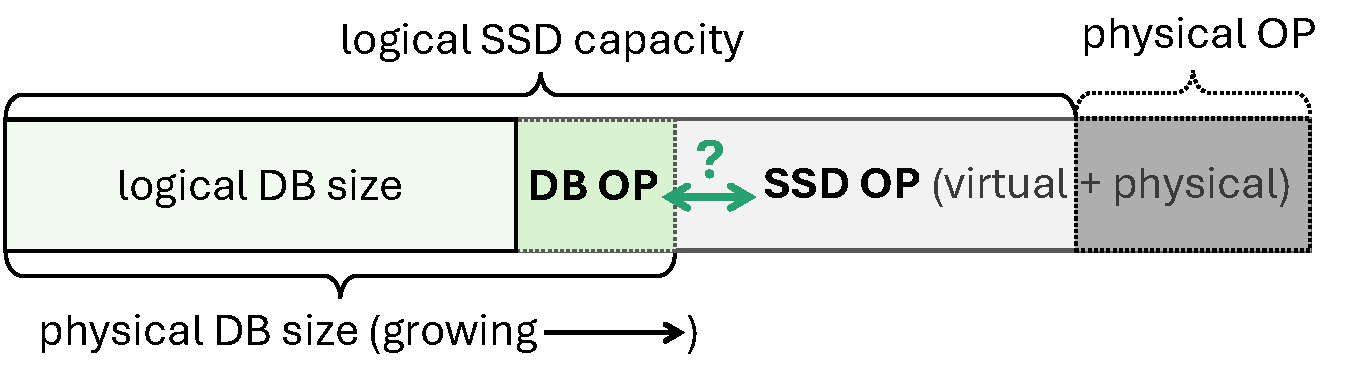
\includegraphics[clip, width=0.9\columnwidth]{figures/op.pdf}
\end{center}
% inline figure

\module{Why total WAF matters.}
Based on this OP split, DB WAF and SSD WAF vary inversely as they contend for OP space, and total WAF varies accordingly.
As shown below, as the physical dataset size increases, DB WAF goes down but SSD WAF goes up:
\begin{center}
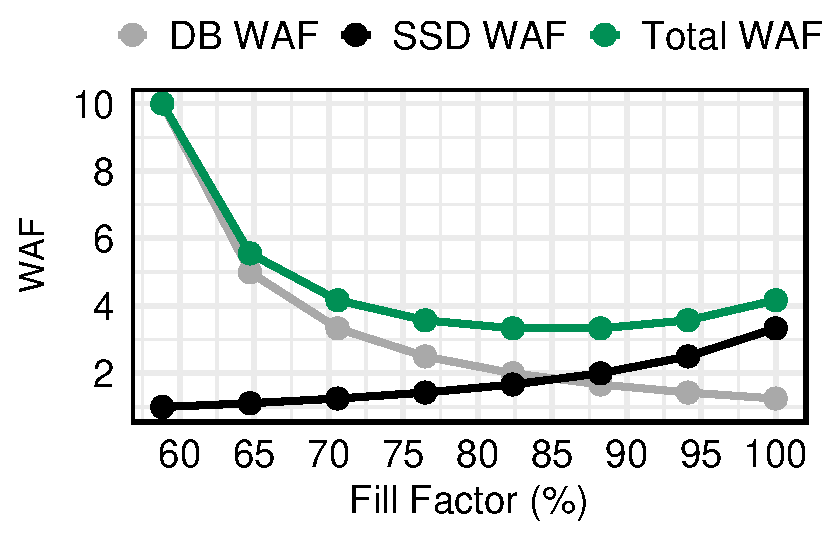
\includegraphics[clip, width=0.6\columnwidth]{figures/opwaf.pdf}
\end{center}
Now, if we aim solely to minimize DB WAF, then DB GC will use the full logical SSD capacity (100\% on the x-axis). 
This indeed keeps DB WAF relatively low, around 1.3.
However, because the SSD was then deprived of the OP space, the SSD WAF increases to approximately 4.2 in return. 
As a result, even though we intended to reduce WA, the SSD ends up performing 5.46× (1.3 × 4.2) more internal writes. 
This total WAF is worse than when the DB GC is triggered earlier, at an 85\% fill factor, for instance, where the total WAF is 3.3. 
This outcome is counterintuitive from the DBMS perspective, but illustrates what happens when the SSD’s internal behavior is ignored.

\module{The case for total WAF consideration.}
This motivates the total WAF formulation: focusing on individual WAFs is counterproductive when reducing one worsens another. 
Thus, total WAF (DB WAF × SSD WAF) better reflects the true cost by representing the total flash writes per transaction. 
We argue that considering total WAF is a key contribution of this work, 
whereas prior studies typically examine WA only within individual layers. 
WA should therefore be analyzed across layers---i.e., as total WAF---rather than in isolation.

\module{Why DBMS, and not SSDs or filesystems?}
To effectively address total WAF, we argue that the DBMS---rather than the filesystem or the SSD---should take the lead.
This may sound counterintuitive, as filesystems and SSDs sit closer to the lower layer and therefore seem better positioned to optimize it.
Moreover, the storage community has made relentless efforts to minimize SSD WAF, and it remains an active research topic today.
However, despite this radical shift, we claim that the DBMS is more suited to, and therefore should, optimize SSD writes for two main reasons.
First, despite extensive research, our prior work shows that most enterprise SSDs still exhibit surprisingly high WAF~\cite{ssdiq}.
Second, the DBMS has the greatest visibility into workload behavior, whereas filesystems and commodity SSDs have virtually none.

%% workload knowledge 
\module{Modern SSDs still exhibit high WAF.}
Our prior research~\cite{ssdiq} has shown that, surprisingly, standard commodity SSDs are not capable of interpreting workload characteristics, even for the simplest skewed patterns. 
As a result, they inevitably suffer from high SSD WAF.
As shown in Figure~3 of our prior work~\cite{ssdiq}, we evaluated a two-zone workload by splitting space 90:10\% and using an access pattern of 10:90\%.
Different enterprise SSDs from multiple vendors all exhibited consistently high WAF, ranging from 3 to 4.8, and their WAF trends closely matched the behavior of greedy GC when compared with simulator results.
This clearly suggests that they do not implement intelligent GC algorithms that exploit workload characteristics.

\module{SSDs lack workload knowledge to reduce WA.}
The fundamental reason why it is intrinsically difficult to build intelligent GC inside SSDs is their lack of visibility into the workload~\cite{DBLP:journals/pomacs/LangeNY25}.
Extensive research has attempted to infer workload characteristics inside SSDs to improve GC~\cite{DBLP:journals/pomacs/LangeNY25,DBLP:journals/cacm/LangeNY23,DBLP:journals/pvldb/KangCOL20},
but such inference introduces significant overhead and remains inherently imperfect.
This is one of the key motivations behind proposals such as open-channel SSDs, ZNS, open programmable SSDs~\cite{DBLP:conf/micro/ParkLLBSCC24}, and newer interfaces like multi-stream and FDP.
These interfaces encourage the application to either fully manage the SSD to be workload-aware or at least share valuable workload information with the device~\cite{SNIA_SDC_2025_TotalCostAndPerformanceOfSSDs, SNIA_SDC_2025_OptimizingHyperscaleFlashStorage}.
This indicates that, without some form of host-level coordination---such as what this paper proposes---SSDs alone cannot effectively address this problem.

\module{Filesystems cannot address total WAF.}
Filesystems are also ill-suited for reducing total WAF.
Situated between the DBMS and the SSD, they lack visibility into database-level access patterns and have no control over SSD-internal data placement.
Consequently, they possess neither the workload knowledge required to lower DB WAF nor the low-level interface needed to mitigate SSD WAF~\cite{DBLP:conf/usenix/BjorlingAHRMGA21}.
These limitations are evident even in filesystems explicitly designed to reduce SSD WAF.
For example, prior work shows that RocksDB running on ZenFS consistently achieves lower SSD WAF than RocksDB on F2FS with ZNS support~\cite{DBLP:conf/usenix/BjorlingAHRMGA21}.
Similarly, with FDP-enabled SSDs, SSD WAF is higher when XFS is used, compared to when RocksDB issues FDP placement hints directly without XFS~\cite{fdprocksdb}.
In both cases, filesystem mediation worsens WAF despite device-aware extensions, demonstrating that filesystems cannot match the effectiveness of DBMS-level write control.
Moreover, when the DBMS already employs out-of-place writes, the filesystem contributes little beyond adding an additional layer of indirection and system-call overhead~\cite{DBLP:conf/icde/NguyenL24,DBLP:conf/icit/HinesCA23,DBLP:journals/corr/SearsIG07,DBLP:journals/pvldb/GaffneyPBHKP22}.
While operating systems provide useful abstractions, these features offer limited benefit to a DBMS that already manages its own memory and storage layout.

\module{DBMS, at the highest layer, can mitigate total WAF the most.}
Therefore, we argue that the DBMS is the most suitable layer for mitigating total WAF.
Although this represents a more unconventional departure from the traditional DB-filesystem-SSD three-layer architecture,
the DBMS benefits from operating at the highest layer.
It possesses the richest knowledge of workload behavior at the topmost layer.
Informed by schema structure, access patterns, and query semantics, DBMS GC has far more potential to outperform SSD GC, and thus mitigate total WAF.

\module{Out-of-place writes are inevitable to solve WA.}
To achieve this, switching from in-place to out-of-place writes becomes necessary; without this flexibility, the DBMS cannot tailor writes to workload characteristics.
Once switched to out-of-place writes, the DBMS gains full control over how and when writes are issued,
allowing it to coordinate write patterns with awareness of both application semantics and SSD behavior.
While adopting out-of-place writes does introduce architectural implications for other DBMS components such as logging and recovery~\cite{WObtree},
we claim it is the only way to enable the SSD write optimizations proposed in this paper.
%%%%%%%%%%%%%%%%%%%%%%%%%%%%%%%%%%%%%%%%%%%%%%%%%%%%%%%%%%%%%%%%%%%%%%%%%%%%%%%%%%%%%%%%%%%%%%%%%%%%%%%%%%%%%%%%%%%%
\subsection{When should the DBMS care about WAF?}\label{sec:q2}
\noindent High SSD WAF becomes critical to SSD performance and lifespan under typical OLTP workloads, 
which are characterized by growing dataset sizes (i.e., varying fill factor), high write intensity, and skewed access patterns~\cite{ssdiq, DBLP:journals/pvldb/KangCOL20, Gray1993DebitCredit}.
Below, we explain how each factor influences SSD WAF and throughput, and how our optimizations can affect them.

\module{Case 1: high fill factor.}
First, with respect to fill factor, SSD WAF increases as the SSD becomes more fully occupied.
This behavior explains why the effectiveness of our optimizations depends on the logical dataset size, as shown in \cref{fig:drilldown:a}.
As the dataset occupies a larger fraction of the SSD capacity, SSD WAF naturally increases for in-place-write LeanStore, 
whereas our SSD-level optimizations guarantee SSD WAF~$=1$ regardless of dataset size.
One way to mitigate this effect is to provision substantially more SSD capacity per logical dataset, 
effectively operating the SSD at a lower fill factor by amortizing space cost.
However, under high fill factors, the system inevitably suffers from elevated SSD WAF.

\module{Case 2: high write intensity workload.}
Second, when the DBMS issues writes at a high rate, SSD throughput degrades substantially under high SSD WAF.
Under high write intensity, flash read and program operations are more likely to arrive on busy flash LUNs, 
increasing contention and amplifying the performance penalty of elevated WAF~\cite{lerner2024principles}.
Furthermore, high SSD WAF directly accelerates wear, shortening the SSD’s lifetime.
Thus, the importance of reducing SSD WAF is significantly heightened in high write-intensity conditions.
In this scenario, reducing DB WAF becomes increasingly beneficial, as it lowers the logical write volume to the SSD, 
effectively reducing the write intensity, potentially by half via compression, for instance.


\module{Case 3: skewed write access pattern.}
Finally, SSD WAF can remain high even under explicitly hot/cold--separated workloads.
In our prior study~\cite{ssdiq}, we showed that enterprise SSDs from multiple vendors exhibit \emph{higher} WAF under skewed workloads than under uniform random access.
Figures~3 and~4 in our previous paper~\cite{ssdiq} demonstrate that these SSDs generally lack sophisticated GC mechanisms and therefore incur high WAF unless the hot data fits entirely within their internal write buffers.
As we argue in \cref{sec:GDT}, it is therefore necessary to implement workload-aware GC mechanisms, such as GDT-based GC, at the application layer, since commodity SSDs rarely exploit such workload characteristics effectively.
Thus, if an in-place DBMS generates an extremely skewed write access pattern, it is likely to suffer from increased SSD WAF.
In contrast, DBMSs that perform out-of-place writes exhibit no such correlation, because frequently accessed PIDs are always written to different locations.

%%%%%%%%%%%%%%%%%%%%%%%%%%%%%%%%%%%%%%%%%%%%%%%%%%%%%%%%%%%%%%%%%%%%%%%%%%%%%%%%%%%%%%%%%%%%%%%%%%%%%%%%%%%%%%%%%%%%
\subsection{What if disks are used?}\label{sec:q3}
\noindent \module{Out-of-place writes remain beneficial on disks.}
When running ZLeanStore on traditional hard disks, we expect it to still benefit from the large sequential writes enabled by out-of-place writes.
Additionally, since we propose not only SSD WAF optimizations but also DB WAF optimizations,
ZLeanStore will outperform in-place-write LeanStore, as it reduces logical writes to the device through compression (\cref{sec:comp}) and GDT-based GC (\cref{sec:GDT}).
Furthermore, HM-SMRs are also zoned storage devices; therefore, ZLeanStore can run on top of them with zone-command support (\cref{sec:zns}).
Hence, even with traditional disks, it is beneficial for DBMSs to adopt out-of-place writes (which are mandatory for HM-SMRs) and apply some of our optimizations accordingly.

%%%%%%%%%%%%%%%%%%%%%%%%%%%%%%%%%%%%%%%%%%%%%%%%%%%%%%%%%%%%%%%%%%%%%%%%%%%%%%%%%%%%%%%%%%%%%%%%%%%%%%%%%%%%%%%%%%%%
\subsection{What happens if a filesystem is used?}\label{sec:q4}
\module{Removing the filesystem is no longer unusual.}
In this paper, we assume that the DBMS issues read and write requests directly to the block device, without an intervening filesystem (\cref{fig:oop2}).
Before discussing the implications of introducing a filesystem, it is important to note that writing directly to the block device is not new.
Recent work has shown that filesystems may slow down transaction throughput due to system call overhead
~\cite{DBLP:conf/icde/NguyenL24,DBLP:conf/icit/HinesCA23,DBLP:journals/corr/SearsIG07,DBLP:journals/pvldb/GaffneyPBHKP22, DBLP:journals/tos/AghayevWKNGA20},
especially for small objects typical of OLTP workloads.
Consequently, several research efforts pursue DB--OS co-design by eliminating the filesystem layer entirely when running DBMSs~\cite{DBLP:journals/pvldb/SkiadopoulosLKK21}. 
Accordingly, it is no longer unusual for databases to run directly on top of the block device.

\module{Total WAF when using a filesystem.}
Nevertheless, the traditional configuration places the DBMS above a filesystem rather than directly on the block device.
To evaluate the effect of filesystems on SSD WAF, we conduct separate experiments by running the in-place-write baseline, LeanStore, on top of three different filesystems: ext4, F2FS, and XFS.
We run the same benchmark as in \cref{fig:intro} and report DB WAF, filesystem WAF, SSD WAF, total WAF, and throughput:

\begin{table}[h]
\centering
\footnotesize
\begin{tabular}{l|rrrrr}
\toprule[1pt]\midrule[0.3pt]
\textbf{Filesystem (LeanStore config.)} & \textbf{DB} & \textbf{FS} & \textbf{SSD} & \textbf{Total} & \textbf{OPS} \\
\textbf{} & \textbf{WAF} & \textbf{WAF} & \textbf{WAF} & \textbf{WAF} & \textbf{(K)} \\
\midrule
ext4 (in-place)                         & 2.00 & 1.00 & 2.41 & 4.87 & 212 \\
F2FS (in-place)                         & 2.00 & 1.03 & 2.48 & 5.13 & 199 \\
XFS (in-place)                          & 2.00 & 1.00 & 2.41 & 4.83 & 212 \\
-- (in-place)                           & 2.00 & --    & 2.36 & 4.72 & 237 \\
-- (out-of-place + all opt.)            & 0.62 & --    & 1.00 & 0.62 & 470 \\
-- (out-of-place + all opt.\ $-$\ comp.)& 3.58 & --    & 1.00 & 3.58 & 328 \\
\midrule[0.3pt]\bottomrule[1pt]
\end{tabular}
\end{table}
\noindent
As shown in the table, the filesystem does not improve WAF; in some cases, it even worsens it and reduces throughput due to the additional layer.
Even F2FS, which is widely regarded as flash-friendly, does not address SSD WAF.

\module{Filesystem should participate in mitigating total WAF.}
If a filesystem is used, the filesystem must share responsibility for mitigating total WAF alongside the DBMS.
The filesystem should be the component performing out-of-place writes, as in log-structured filesystems~\cite{DBLP:conf/fast/LeeSHC15, nilfs2, lfs}, and should align its segment size with the SSD’s GC unit.
For in-place DBMSs, the filesystem alone is responsible for mitigating SSD WAF; DB WAF remains unaddressed.
When the DBMS also performs out-of-place writes, DB GC must account for the filesystem’s write patterns when selecting victim zones, after aligning the DBMS’s GC unit with the filesystem’s segment size.

%%%%%%%%%%%%%%%%%%%%%%%%%%%%%%%%%%%%%%%%%%%%%%%%%%%%%%%%%%%%%%%%%%%%%%%%%%%%%%%%%%%%%%%%%%%%%%%%%%%%%%%%%%%%%%%%%%%%
\subsection{What about shared/multi-device scenarios?}\label{sec:q5}
We assume a single-instance, single-device setup in this work.
Oftentimes, especially in cloud environments, storage is shared across instances or spans multiple devices.
Although we do not explore these settings, our optimizations can potentially be applied to such scenarios.
We leave a detailed exploration of shared-device and multi-device environments for future work.

\module{Shared device scenario.}
When multiple database instances share a physical device through a virtualization layer, DB-level WAF mitigation remains the responsibility of each DBMS space manager within the logical capacity exposed by the virtual disk (e.g., VMDK).
The DBMS observes and manages only this guest-visible logical namespace and can track how much logical space it has allocated or left free~\cite{vmware-vsphere-vmfs}.
However, it has no visibility into how these logical allocations map to physical offsets in the datastore or how much physical space is actually consumed.
Consequently, DB-level WAF and SSD-level WAF are addressed at different layers of the stack.
At the DB level, the space manager must decide whether to consume remaining logical free space (implicitly relying on physical headroom) or to reclaim already used space earlier to control DB-level WAF.
SSD-level WA mitigation, in contrast, requires coordination below the guest boundary.
The virtualization layer’s storage subsystem (e.g., the VMFS layer managing VMDKs) could be extended to support out-of-place writes across VMs, maintain a global view of write streams issued by different tenants, and allocate physical space according to our proposed optimizations, including aligning GC units (\cref{sec:gcgranularity}) and adopting the NoWA pattern (\cref{sec:nowa}).
Additionally, if the hypervisor and device stack expose FDP to guests, FDP hints could be propagated through the virtualization layer to the device~\cite{SNIA_SDC_2025_SSDVirtualization}.

\module{Multi-device scenario.}
When multiple SSDs are used and the DBMS directly manages them, the space manager should coordinate usable space and garbage collection across devices to optimize DB-level WAF.
This configuration gives the DBMS greater flexibility, since garbage collection can be managed independently on each device while balancing logical utilization across them.
For SSD-level WAF optimizations, the device manager should locally track the active-group history on each device to preserve the NoWA pattern.
If multiple SSDs are abstracted as a single logical block device by RAID or an array controller, the DBMS no longer retains ownership of physical placement decisions, and coordination across devices is therefore handled by the storage subsystem.
For instance, in multi-SSD storage systems such as ONTAP~\cite{DBLP:conf/fast/Curtis-MauryKRM24} and FlashArray~\cite{PureStorageFlashArrayArchitecture}, a centralized storage-controller placement and space-management layer (e.g., WAFL in ONTAP) is the natural layer to implement our SSD-level WAF optimizations.

%%%%%%%%%%%%%%%%%%%%%%%%%%%%%%%%%%%%%%%%%%%%%%%%%%%%%%%%%%%%%%%%%%%%%%%%%%%%%%%%%%%%%%%%%%%%%%%%%%%%%%%%%%%%%%%%%%%%
\subsection{Is doublewrite buffering really necessary?}\label{sec:q6}
In \cref{sec:oop}, we use the avoidance of doublewrite buffering as one motivation for advocating out-of-place writes instead of in-place updates.
We address three main aspects of doublewrite buffering.

\module{DWB is enabled by default.}
First, doublewrite buffering is enabled by default in InnoDB to ensure data integrity.
According to the MySQL reference manual, it should only be disabled when performance is prioritized over durability~\cite{mysql-dwb}.
Without it, InnoDB cannot recover from torn-page failures caused by power loss during a page write.
Although a checksum mismatch enables corruption detection, recovery requires an intact page copy.
For this reason, we use doublewrite buffering as the baseline.

\module{DWB exists across many systems.}
Second, this mechanism is not unique to MySQL.
Many systems employ similar techniques to guard against torn writes.
PostgreSQL, for example, logs a full-page image on the first modification after each checkpoint (\emph{full-page writes})~\cite{postgresql/doc/dwb},
and SQLite preserves the old page in its rollback journal~\cite{sqlite-journal}.
Other systems, such as CedarDB~\cite{cedardb-dwb}, XtraDB~\cite{xtradb-dwb}, and MariaDB~\cite{mariadb-dwb}, also use doublewrite buffering.
By contrast, SQL Server~\cite{sqlserver-pageverify} and Oracle~\cite{oracle-block-checksum} detect but cannot automatically recover from torn-page writes.
Even AWS provides page-level atomic writes on EC2 instances to allow doublewrite buffering to be safely disabled~\cite{aws-dwb}.

\module{Hardware/OS may not guarantee atomicity.}
Finally, hardware-level atomicity is insufficient.
Even when bypassing the filesystem and writing directly to NVMe devices,
atomicity is guaranteed only at the sector level (typically 512~B, as in most SSDs used in our experiments, or 4~KiB)~\cite{nvmexpress-spec-1.1}.
Database pages are much larger (e.g., 16~KiB in MySQL and 8~KiB in PostgreSQL),
so torn pages remain possible.
Moreover, PostgreSQL relies on the OS page cache (i.e., buffered I/O by default), so atomicity also depends on the filesystem implementation.

All of these concerns are eliminated once the system adopts out-of-place writes.

%%%%%%%%%%%%%%%%%%%%%%%%%%%%%%%%%%%%%%%%%%%%%%%%%%%%%%%%%%%%%%%%%%%%%%%%%%%%%%%%%%%%%%%%%%%%%%%%%%%%%%%%%%%%%%%%%%%%
\subsection{How can we calculate DB WAF on other DBMSs?}\label{sec:q8}
In the total WAF formulation, SSD WAF is relatively straightforward to obtain by comparing the physical flash writes reported via OCP commands with the logical writes issued by the DBMS to the SSD (if the SSD supports them).
In contrast, computing DB WAF is often less clear, as it is nontrivial to distinguish necessary user writes from redundant writes.
In this paper, we define user writes as the sum of eviction writes and checkpoint writes, assuming that the maximum WAL file size equals the buffer pool size.
Different DBMSs implement checkpointing differently and may incur additional writes due to system-specific mechanisms (e.g., RocksDB compaction) or writing strategies (e.g., in-place versus out-of-place updates).
In this section, we describe how DB WAF is calculated for four systems: MySQL/InnoDB, PostgreSQL, WiredTiger, and RocksDB.
We assume that all WAL logs are stored on a separate device, consistent with \cref{fig:intro}.

\module{DB WAF of MySQL/InnoDB.}
As mentioned and evaluated in \cref{sec:intro}, MySQL’s doublewrite mechanism largely determines the DB WAF, similar to in-place-write systems such as the in-place LeanStore baseline.
Before flushing dirty pages from the LRU list or the flush list in the buffer pool, InnoDB first copies each full page into the DWB~\cite{mysql-dwb}.
The pages are then written sequentially to the DWB area on disk and subsequently written again to their final locations in the tablespace.
The size of the DWB is configured by the number of doublewrite files and the number of pages per doublewrite batch (e.g., \texttt{innodb\_doublewrite\_files} and \texttt{innodb\_doublewrite\_pages}).
This space is allocated per buffer pool instance, resulting in only a few megabytes of doublewrite space per instance under default settings~\cite{mysql-sourcecode}.
If the same page is selected for flushing multiple times before the DWB itself is persisted, InnoDB coalesces these requests and retains only the most recent page image in the DWB, avoiding redundant writes within a single doublewrite batch.
Furthermore, with respect to checkpoint writes, InnoDB exposes the maximum redo log size as a configurable parameter~\cite{mysql-checkpoint}.
When this parameter is set sufficiently large, checkpointing is no longer forced by log-space pressure and thus avoids unnecessary checkpoint-induced page flushes.
Consequently, the DB WAF can be expressed as follows:
\[
\text{WAF}_{\text{MySQL}} =
\frac{\text{LRU list flushes} + \text{flush list flushes} + \text{DWB}}
     {\text{LRU list flushes} + \text{flush list flushes}}
\]

\module{DB WAF of PostgreSQL.}
Unlike MySQL, PostgreSQL implements doublewrite protection via full-page writes to the WAL rather than a separate doublewrite file~\cite{postgresql/doc/dwb},
which amplifies WAL traffic and increases checkpoint frequency.
This behavior is particularly harmful for OLTP workloads with small updates, where the amount of data modified per page flush is typically much smaller than the page size~\cite{nvppl}.
As full-page writes indirectly amplify user writes, we derive the DB WAF for PostgreSQL as follows.
First, we run PostgreSQL with full-page writes disabled and tune the checkpoint frequency such that the WAL size remains proportional to the buffer pool size, since the maximum WAL size is not strictly enforced.
Under this configuration, we measure the ratio of eviction writes to checkpoint writes and infer the amount of checkpointing required to truncate the WAL.
Second, we enable full-page writes and measure eviction and checkpoint writes.
Using the previously obtained ratio, we estimate the checkpointing required for the observed eviction writes and attribute the remaining checkpoint writes to full-page writes.
We define the DB WAF for PostgreSQL as follows:
\[
\text{WAF}_{\text{Postgres}} =
\frac{\text{eviction} + \text{checkpointing (including full-page)}}
     {\text{eviction} + \text{required checkpointing}}
\]
Here, we exclude vacuuming- and pruning-induced writes~\cite{PostgreSQLDoc}, as PostgreSQL’s out-of-place version updates primarily incur index-level WA rather than page-level WA.

\module{DB WAF of WiredTiger.}
For out-of-place-write systems, DB WAF primarily arises from space reclamation rather than doublewrite buffering.
In WiredTiger, checkpoints identify unreferenced pages and return their blocks to the free list~\cite{WiredTiger_Checkpoint_Arch}.
If space reclamation proceeds too slowly, data files may grow without bound and eventually exhaust available storage~\cite{MongoDB_WiredTiger_DataSize_Increase_2021}.
Although manual invocation of \texttt{compact()} can reclaim space by rewriting live pages and truncating files~\cite{wiredtiger-compaction}, our separate experiments show that this incurs substantial overhead.
We define DB WAF for WiredTiger in terms of space reclamation overhead.
Let required checkpointing be the minimum checkpoint-induced write volume under a dirty-page-to-log-write ratio with a buffer-pool-sized WAL.
Any checkpointing beyond this minimum is attributed to space reclamation and considered DB WAF.
If \texttt{compact()} is used, its write volume can be counted as space reclamation overhead in place of the excess checkpoint writes.
Accordingly, we define the DB WAF for WiredTiger as:
\[
\text{WAF}_{\text{WiredTiger}} =
\frac{\text{eviction} + \text{checkpointing} + \text{compact}}
     {\text{eviction} + \text{required checkpointing}}
\]


\module{DB WAF of RocksDB.}
In RocksDB, DB WAF arises from LSM-tree compaction.
Each update is written to both the memtable and the WAL, and when the active memtable exceeds its flush threshold, it becomes immutable and is flushed to a level-0 SST file. 
Whether that flush triggers a cascade of compaction writes depends on the compaction strategy and thresholds such as the L0 file-count trigger, level size targets, and target SST file sizes~\cite{rocksdb_db_bench}.
As a result, LSM-tree-driven DB WAF varies significantly with such compaction policies and parameters, as extensively studied in prior work~\cite{LSMTreeCost_SIGMOD2024, Dayan_TODS2018, Liu2025_ArceKV, lsmdesign, Dayan_VLDB2022_Hybrid}.
Therefore, these configurations should be tuned to workload characteristics. 
It is important to note that RocksDB is not page-based, unlike the three systems above.
Thus, its DB WAF is not directly comparable to theirs.
Nevertheless, we define the DB WAF for RocksDB as follows:
\[
\text{WAF}_{\text{RocksDB}} =
\frac{\text{memtable flush} + \text{compaction}}
     {\text{memtable flush}}
\]
